\documentclass{sigchi}

% Arabic page numbers for submission. 
% Remove this line to eliminate page numbers for the camera ready copy
%\pagenumbering{arabic}

% Load basic packages
\usepackage{balance}  % to better equalize the last page
\usepackage{graphics} % for EPS, load graphicx instead
\usepackage{times}    % comment if you want LaTeX's default font
\usepackage{url}      % llt: nicely formatted URLs

% Load basic packages
%\usepackage[pdftex]{graphicx}
%\usepackage{amsmath, amssymb}
\usepackage{verbatim}
%\usepackage{tabularx}
\usepackage{mdwlist} %compact lists
%\usepackage{algorithm}
%\usepackage{algpseudocode} % program code

\usepackage{listings}

% llt: Define a global style for URLs, rather that the default one
\makeatletter
\def\url@leostyle{%
  \@ifundefined{selectfont}{\def\UrlFont{\sf}}{\def\UrlFont{\small\bf\ttfamily}}}
\makeatother
\urlstyle{leo}


% To make various LaTeX processors do the right thing with page size.
\def\pprw{8.5in}
\def\pprh{11in}
\special{papersize=\pprw,\pprh}
\setlength{\paperwidth}{\pprw}
\setlength{\paperheight}{\pprh}
\setlength{\pdfpagewidth}{\pprw}
\setlength{\pdfpageheight}{\pprh}

% create a shortcut to typeset table headings
\newcommand\tabhead[1]{\small\textbf{#1}}

% to give it a fighting chance of not being over-written, 
% since its job is to redefine many LaTeX commands.
\usepackage{ifpdf}
\ifpdf
\usepackage[pdftex]{hyperref}
\else
\usepackage{hyperref}
\fi
\hypersetup{
pdftitle={SIGCHI Conference Proceedings Format},
pdfauthor={LaTeX},
pdfkeywords={SIGCHI, proceedings, archival format},
bookmarksnumbered,
pdfstartview={FitH},
colorlinks,
citecolor=black,
filecolor=black,
linkcolor=black,
urlcolor=black,
breaklinks=true,
}

\graphicspath{{pictures/}}

% Use this command to override the default ACM copyright statement (e.g. for preprints). 
% Consult the conference website for the camera-ready copyright statement.
 \toappear{\scriptsize Permission to make digital or hard copies of all or part of this work for personal or classroom use is granted without fee provided that copies are not made or distributed for profit or commercial advantage and that copies bear this notice and the full citation on the first page. Copyrights for components of this work owned by others than the author(s) must be honored. Abstracting with credit is permitted. To copy otherwise, or republish, to post on servers or to redistribute to lists, requires prior specific permission and/or a fee. Request permissions from Permissions@acm.org. \\
 {\emph{UIST'13}}, October 8--11, 2013, St. Andrews, United Kingdom. \\
 Copyright \copyright~2013 ACM 978-1-4503-2268-3/13/10...\$15.00. \\
http://dx.doi.org/10.1145/2501988.2502007}
 
\clubpenalty=10000 
\widowpenalty = 10000 


\newcommand{\eg}{e.g.,\ }
\newcommand{\ie}{i.e.,\ }
\newcommand{\haiku}{Haiku~OS}
\newcommand{\wysiwyg}{\mbox{WYSIWYG}\ }
\newcommand{\dragndrop}{drag and drop\ }


% End of preamble. Here it comes the document.
\begin{document}

\title{Lablet: A Mobile Learning Enviornment}

\numberofauthors{1}

\author{
	\alignauthor \mbox{Clemens Zeidler, Anna Yang, Kasper van Wijk}\\
		\affaddr{University of Auckland}\\
		\affaddr{38 Princes Street}\\
		\affaddr{Auckland 1010, New Zealand}\\
		\email{\{clemens.zeidler, a.yang, k.vanwijk\}@auckland.ac.nz}
}

\maketitle

%\tableofcontents

\begin{abstract}
%TODO Anna
\end{abstract}

\category{H.5.2}{User Interfaces}{Graphical user interfaces (GUI)}


\keywords{e-learning; mobile devices; physics experiments; electronic handouts}


\section{Introduction}
%Kasper: What do our (or any physics department's) labs aim to accomplish now (on paper), what does the lablet provide/add? Sensing, and analysis capabilities would be the two main things.
%A connection with "modern wired life" (there may be  a better term) is maybe another important consideration.
The increasing ownership and availability of mobile devices with advanced sensors equip anyone interested in physics to get creative with scientific inquiries.
The Auckland Lablet provides an active learning environment for Physics experimentation on an Android tablet.
The intuitive interface and the rich sensor suite of touch screen tablets create a powerful learning tool built on commodity hardware.
Students use Lablet to capture and analyse data in and outside our teaching laboratories; the Lablet modules leverage a range of internal sensors in the tablet, and the fully customisable Lablet environment guides students through activities and experiments.

Students use familiar technology to optimise their time with learning hands-on Physics with Lablet.
In addition, Lablet creates a “paperless workflow” for grading and student feedback, so that the Lablet maximises the time our staff spend interacting with students.

We hope a community of Lablet users will grow a home in high schools, studio-based learning environments, and flipped classrooms.
Lablet’s low cost and versatility create a wealth of opportunities for playful independent exploration.
Imagine students combining Doppler analysis and video motion tracking data of cars on a busy road, using an accelerometer in an elevator to measure the height of a building, or analysing the motion of a ball on a sport field.

The Auckland Lablet is open source; our applications and source code are freely available for use and modification.
The current release includes video, audio and accelerometer capturing and analysis modules.
Future releases will exploit the ambient light sensors, compasses, gyroscopes and GPS receivers found in tablets, as well as purpose-built Arduino-based Bluetooth connected sensors.


\subsection{Contributions}

\begin{itemize*}
\item Description of Lablet a new Mobile learning environment that supports multiple sensors.
\item Possible experiments and analyses.
\item Introduction a scripting language to customize Lablet's lab activies.
%\item Evaluation of Lablet.
\end{itemize*}


\section{Related Work}
While mobile technologies offer opportunities to transform teaching and learning practices~\cite{karnad2014trends, Kukulska2010}, relatively few mobile projects have been designed that could facilitate social learning and user-generated content~\cite{Frohberg2009}.


%TODO (Anna):
\cite{Kearney2012}
\cite{Etkina2006}
\cite{Millar2002}
\cite{Trumper2003}


% camera:

The camera sensor can be used to record a video of an experiment and by using video analysis software various measurements can be made.
% Web camera as a measuring tool in the undergraduate physics laboratory and Investigating viscous damping using a webcam 
For example, a web camera has been used to analyze diffusion of ink drop in water, damped oscillations of a pendulum, diffraction patterns~\cite{Nedev2006} and mass oscillating in a viscous fluid~\cite{Shamim2010}.

% Cellular Phones Helping To Get a Clearer Picture of Kinematics 
The kinematic of a water jet from a hose can be studied by taking a photo of the scene using a mobile device~\cite{Falcao2009}

% sound:

% acoustics
Using a fast Fourier transformation the different types of sounds such as a tone, a periodic and none-sinusoidal vibration pattern, noise and impulse can be analyzed using the microphone of a mobile device~\cite{KuhnAcousticPhenomena2013}.

% accustic measurement of a bouncing ball
Mobile devices can also be used to record the sound of an bouncing ball~\cite{Schwarz2013Acoustic}.
From the time difference of the bounces and the initial height the gravitation can be determined.

% bell-jar
The sound propagation in vacum can be demonstrated by hanging a ringing mobile phone into bell-jar~\cite{CaleonBellJar2013}.


% accelerometer:

% Analyzing free fall with a smartphone acceleration sensor
Another experiment proposes to facilitate the accelerometer of a mobile device to analyze a free fall by dropping the mobile device on a cushion~\cite{VogtFreeFall2012}.
% Analyzing spring pendulum phenomena and radial acceleration with a smartphone acceleration sensor
Similar, a mobile device can be used to record acceleration of a spring pendulum, a coupled spring pendulum~\cite{KuhnPendulum2012}, a free and a damped harmonic oscillation~\cite{Castro2013}.
By rotating the mobile device the radial acceleration can be measured~\cite{VogtRadialAcc2013}.


% other sensors:

% The optical mouse for harmonic oscillator experimentation
An optical mouse can be used as an extremely cost-effective displacement sensor, for example, to measure the damped harmonic oscillations~\cite{Ng2005}.

% oscilloscope
Mobile devices can be act a portable oscilloscopes~\cite{Forinash2012}.
The microphone jack can be used as an input.
The recorded data can be Fourier analyzed.

% Smartphones—Experiments with an External Thermistor Circuit
The microphone jack can also be used as an input for external sensors such as a thermistor~\cite{Forinash2012}.

% Wiimote
The Wiimote sensor can been used to track multiple objects simultaneously, \eg to observe a spring system with multiple coupled masses~\cite{Skeffington2012}.

% A simple demonstration for exploring the radio waves generated by a mobile phone
A mobile phone can also be used as a radio wave source that can be measured using a simple wave detector~\cite{Hare2010}.

\section{Sensors}
% recording and sensors
Lablet is designed to simultaneously record data from multiple sensors.
This allows to record, for example, a video and accelerometer data at the same time.
Currently Lablet supports common sensors in mobile devices, \ie camera, microphone and accelerometer.
However, Labet's architecture makes it easy to support other sensors in the future.
Before starting an experiment the user can select what sensors should be used when recording.

\subsection{Camera}
Lablet gives experimenters the options to record a video at different resolutions and frame rates.
The usual recording frame rate of modern mobile devices is between 25 and 30 fps.
Compared to a classic experiment where experimenters use a stopwatch to measure the time this allows a more precise measurement with an accurency smaller 50ms.

% slow experiments
However, some experiments run for multiple hours.
For these long experiments it is not practical to record a video at a high frame rate and high video resolution since this results in very large video files.
For example, using Lablet to record a video at 1280x800@30fps results in a mp4 file roughly of the size of 4.2 Gb per hour.
In order to reduce the disk requirements Lablet allows to lower frame rate and video resolution.
If for an experiment the video resolution is less important than the time resolution one should just lower the video resolution.
On the other hand if a high video resolution is required one can lower the frame rate.
Lablet allows to record video with a video frame rate down to 0.1 fps but theoretically there is now lower limit for the recording frame rate.

\subsection{Microphone}
Lablet uses the build in microphone of a mobile devices to record audio data.
The use sampling rate is 44100Hz.
This allows the recording of sound in the human hearable range of roughly 20Hz - 20000Hz.

\subsection{Accelerometer}
The build in a accelerometer of mobile devices usually provide accelerometer data for x, y and z direction.
%TODO: The readout frequency is between...
%TODO: The precision is in the range of...
Lablet calculate a resulting total acceleration value from these three vales
\[
a_{total} = \sqrt{a_x^2 + a_y^2 + a_z^2}
\]

\section{Analysis}
Once sensor data has been recorded it can directly be analyzed within Lablet.
While the architecture of Lablet allows to analyze a certain data set with different analysis modules there is currently only on analysis module available for each sensor.
Once the analysis has be completed the data as well as the analysis results can be exported.

\subsection{Motion Analysis}
The motion analysis module can be used to analyze the trajectory of a moving object.
Therefore, the experimenter first has to calibrate the size of the the recorded video and then has to step throw the video frame by frame to marks the position of the moving object.
From this position data the velocity and the acceleration can be derived.

% crop video length
In general the recorded video is longer than the experiment, \ie it starts before and ends after the experiment.
For that reason, before doing the actual analysis, the video should be cropped to the desired length.
This can be done on a video settings screen (see Figure~\ref{fig:MotionAnalysisSettingsScreen}).
On that screen also the analysis frame rate can be adjusted.
This can be used to reduce the number of frames that has to be considered in the analysis.

\begin{figure}[ht]
\centering
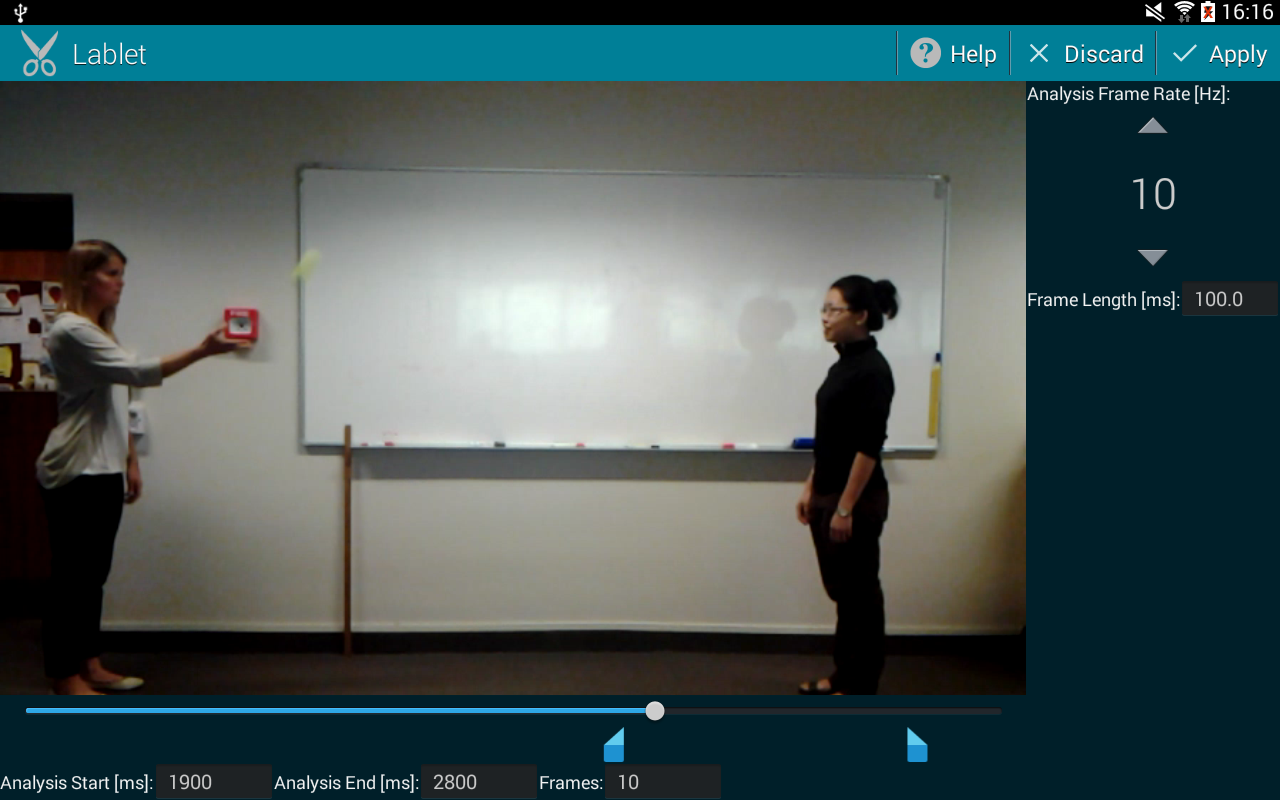
\includegraphics[width=.99\columnwidth]{MotionAnalysisSettings}
\caption{Motion analysis settings screen.
On the left bottom the part of the video that contains the experiment can be selected.
On the right side the analysis frame rate can be adjusted.\label{fig:MotionAnalysisSettingsScreen}
}
\end{figure}

% length scale 
To determine the distance and extend of objects in video scene is very difficult if no additional informations are given.
To solve this problem has a length scale that can be put on top of a reference object with known size.
By entering the length of the marked reference object the size of the scene is calibrated (see Figure~\ref{fig:MotionAnalysis}).
% how to get optimal results
Note that this assumes that the video is recorded parallel to the plane of the moving object.
Furthermore, to ensure a proper calibration the reference object should be located on that plane as well.

% orientation
Optional, to complete the video scene calibration the origin and rotation of can be adjusted.
To do so Lablet has a coordinate system that can be moved and rotated on the screen (Figure~\ref{fig:MotionAnalysis}).


\begin{figure}[ht]
\centering
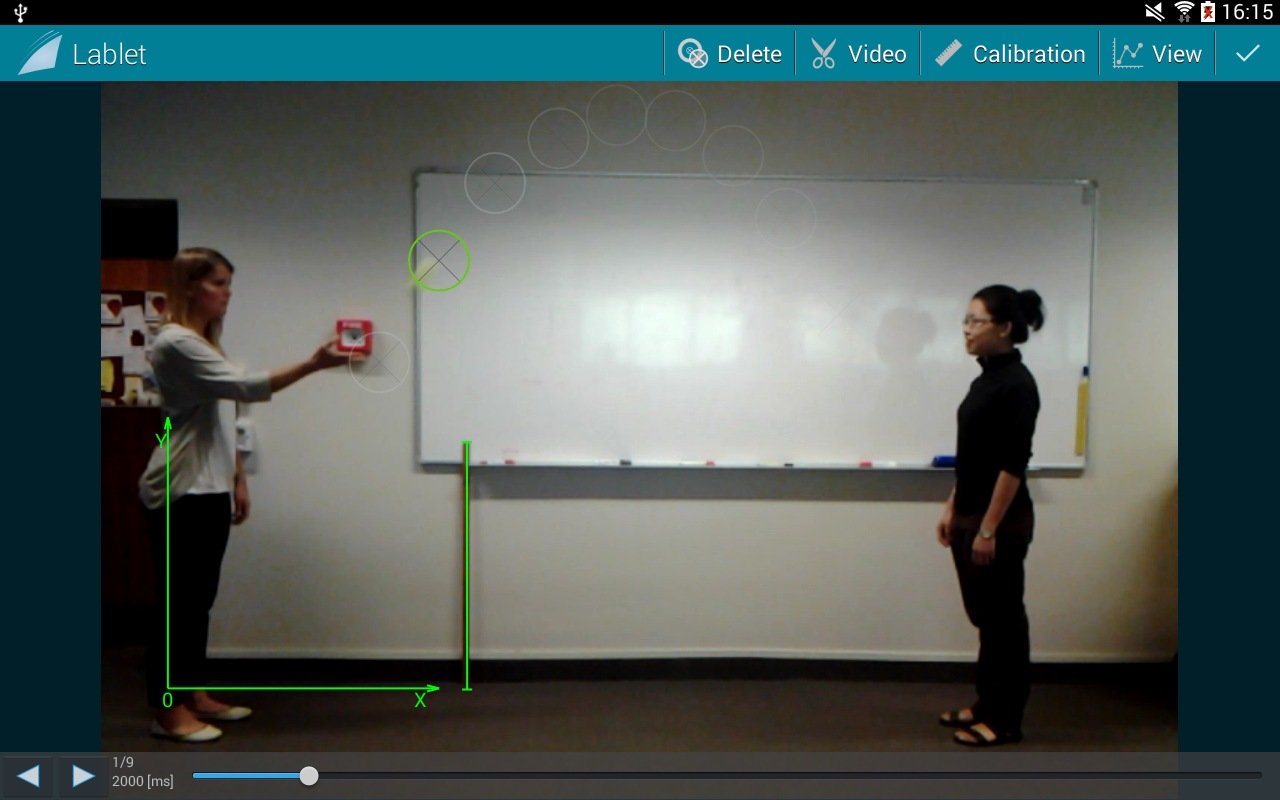
\includegraphics[width=.99\columnwidth]{MotionAnalysis}
\caption{Motion analysis screen.
The green length scale can be used to calibrate the size of the video scene.
The coordinate system can be used to set origin and orientation of the video scene.\label{fig:MotionAnalysis}
}
\end{figure}

\subsection{Frequency Analysis}
The Frequency analysis module does a Fourier analysis of recorded audio data.
This is done by parting the audio data into windows of fixed size.
For each window first a Hamming window function is applied and then a discrete Fourier analysis is performed.
The resulting frequency spectrum is plotted in a time frequency graph (Figure~\ref{fig:FrequencyAnalysis}).
The window size as well of as the window overlap can be adjusted to optimize the output.
A window overlap of 0\% means that the windows are in a consecutive line while an overlap of 50\% means that the last half of the previous window is the first half of the following window.
Sometimes frequency changes are very subtle and changing the colour contrast and brightness can help to make small change more visible.
The time frequency plot is zoomable to look at interesting points in detail. 

\begin{figure}[ht]
\centering
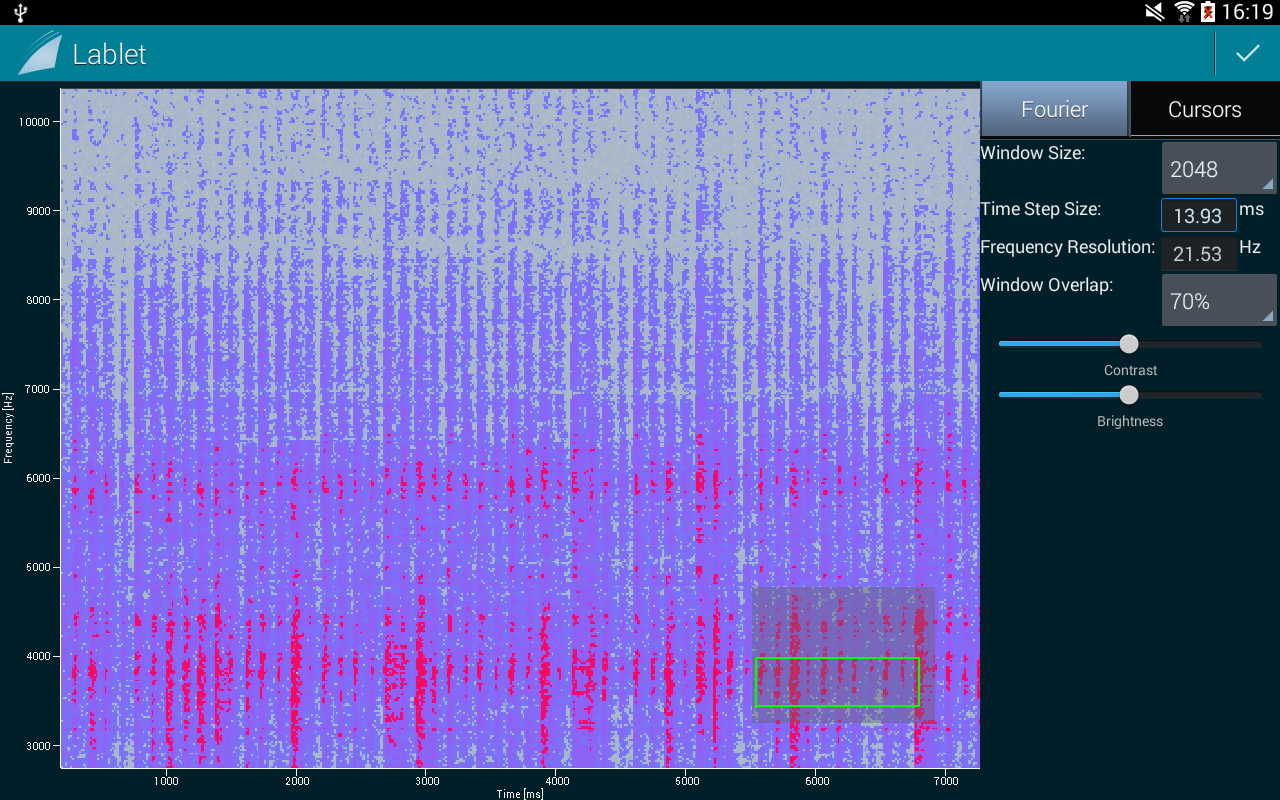
\includegraphics[width=.99\columnwidth]{FrequencyAnalysis}
\caption{Frequency analysis screen.\label{fig:FrequencyAnalysis}
}
\end{figure}

% what window size and window overlap do
At a sampling rate $f_s$ and a window size $n$ samples time between two windows is
\[
\Delta t_w = n / f_s
\]
This means the time resolution of the time frequency plot is high if the window size is small.
When using a percental window overlap $p$ this time deceases further to
\[
\Delta t_w = n / f_s * (1 - p / 100)
\]
Note, that when using a window overlap only existing data is reused thus no new information is used when increasing the window overlap.
However, since a hamming window function is indeed sense to use a window overlap and in practice some frequency changes become more visible at certain window sizes.

% frequency resolution
%TODO: is frequency resolution the right term?
The frequency resolution is given by
\[
\Delta f = f_s / (n - 1)
\]
Thus, the trade-off of increasing the time resolution by decreasing the window size is that the frequency resolution degrades.
In practice a good compromise has to be found that gives good results for a certain problem.

% cursors
Lablet allows to mark an arbitrary number of points on the time and the frequency axis.
This can, for example, be used to measure the time distance between two audio signals or the frequency difference of a Doppler shift experiment.
These marked points can be exported for further analysis.

\subsection{Accelerometer Analysis}
Lablet automatically integrates the measured accelerometer data to get velocity and displacement of the device.
To do so we assume the mobile device is initially at rest and only gravity is affecting it.
Ususaly the measured total acceleration at rest is not equal to the earth gravity $g$ and the value has to be calibrated.
The experimenter can do this by placing a calibration line in the time acceleration graph (Figure~\ref{fig:AccelerometerAnalysis}).

% problem
Integrating the acceleration is a very difficult task and small errors in the initial acceleration results in a drift of the integrated data.
This becomes even worse when doing the the second integral.
Because of that one can't expect accurate but only qualitative results for velocity and distance.

% elevator example and discussion
The accelerometer data in Figure~\ref{fig:AccelerometerAnalysis} shows a journey in an elevator from the top of the building to the ground floor.
The first peek shows how the elevator accelerates till it reach a certain speed then the second peek indicates how the elevator decelerates to come to a stop at the bottom of the building.
If one would place the calibration line in the time acceleration graph without looking at the integrals it is almost certain that velocity and distance graphs have a large drift.
To avoid this problem one can use the knowledge that the lift was at rest at the top and at the bottom of the journey.
Fiddling with the calibration line till the velocity graph shows a velocity of zero at the beginning and the end results in a traveled distance that is actually compatible with the height of the building.

\begin{figure}[ht]
\centering
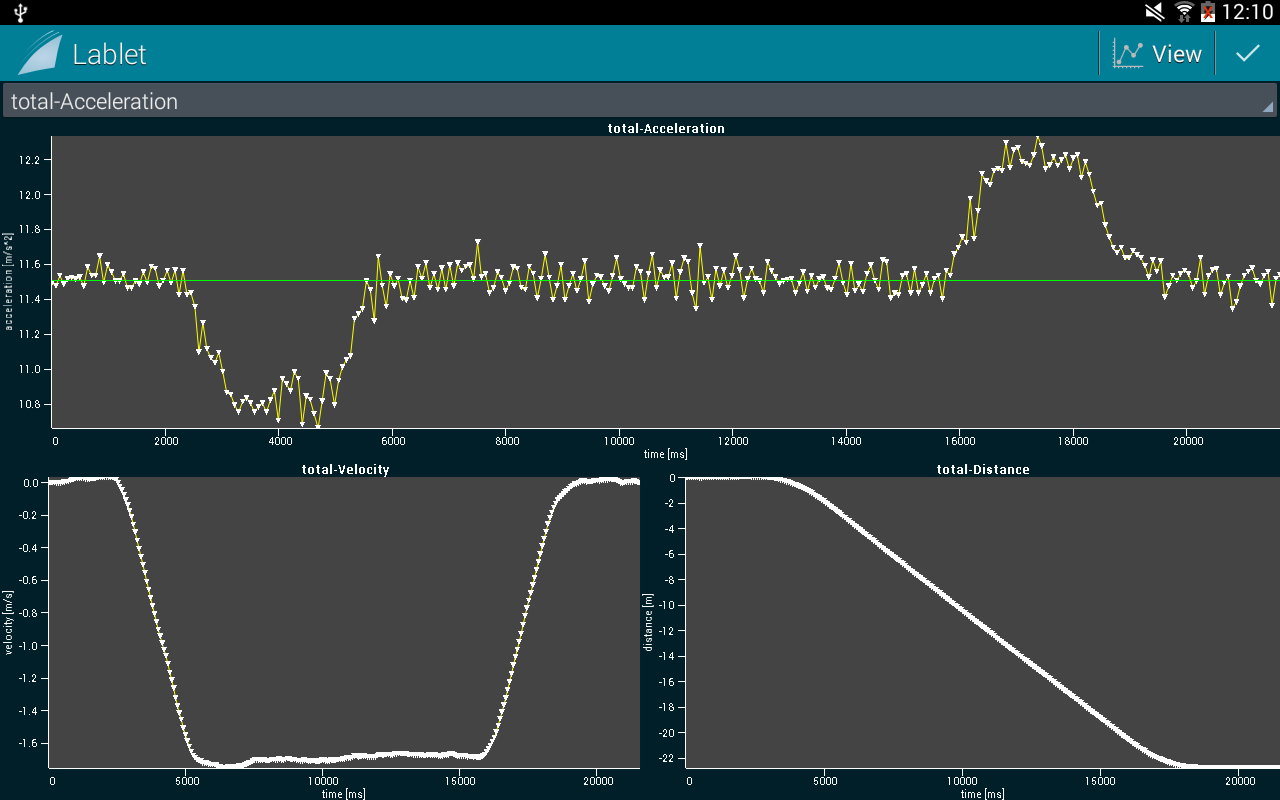
\includegraphics[width=.99\columnwidth]{AccelerometerAnalysis}
\caption{Accelerometer analysis screen.
In the top time acceleration the experimenter can calibrate the initial acceleration at rest.
From this the velocity and distance graphs are calculate (bottom left and bottom right).\label{fig:AccelerometerAnalysis}
}
\end{figure}

\section{Lab Activities}
In a classical laboratory class students usually get a paper-based handout that guides them through the class.
The handout can include instructions, questions and other tasks.
For example, the handout can instruct students to manually calculate the velocity of a moving object using Lablet's motion analysis module.
The desired learning outcome for this experiment could be to understand how to calculate the velocity from consecutive position measurements and discuss the velocity time graph.
To do so data can be exported from the mobile device and analyzed on a computer.
However, this complicates the laboratory class since more equipment is required and students needs to learn to use the analysis software.
Another way to analysis the data is to calculate the velocity manually using pen, paper and a calculator.
The drawback of this method is that students have to repeat a relative simple task multiple time and the results and because teachers have to recalculate the results they are difficult to verify.
Either way, students have to spend time with tasks that are not part of the desired learning outcome.

% Lablet's solution
Lablet solves this shortcomings described above by providing a way to run {\em Lab Activities} tailored for individual laboratory classes.
A Lab Activity can include a multitude of elements such as instructions, quesitions, experiments, visualization of experiment data or advanced analysis task.

\begin{figure}[ht]
\centering
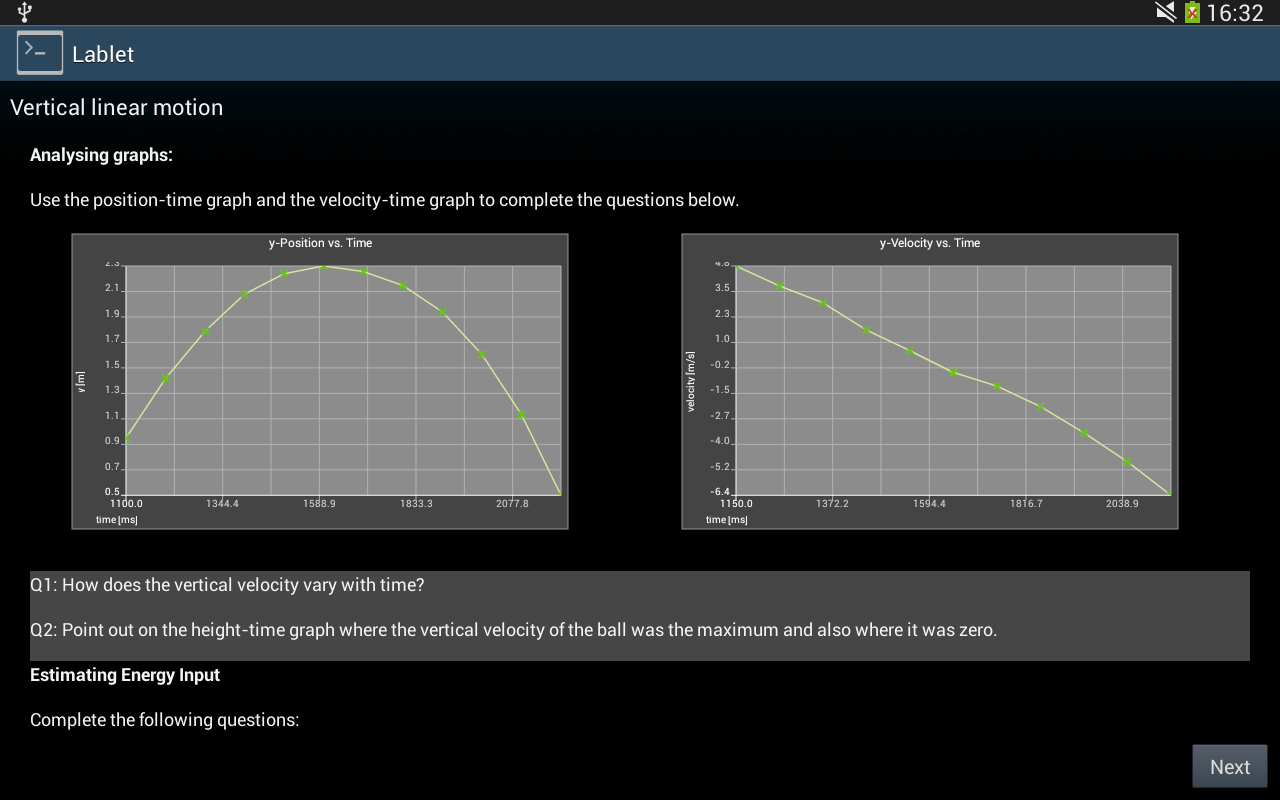
\includegraphics[width=.99\columnwidth]{LabActivitySheet}
\caption{Sheet from a Lab Activity containing various different elements.\label{fig:LabActivitySheet}
}
\end{figure}

% desciption of the Lab Activities UI
Each Lab Activity can have multiple sheets.
The sheets are in a horizontal layout and students can go to next or previous sheet using a swipe gesture.
Each sheet can have an unlimited number of elements.
Some elements requires to be completed before students can proceed to the next sheet.
For example, check boxes needed to be ticked before the next sheet becomes available.
Figure~\ref{fig:LabActivitySheet} shows an example of a single sheet containing various different elements.

% layout
Lablet comes with a powerful but simple layout model to position elements on a sheet.
Elements can be placed in horizontal or vertical boxes.
Vertical and horizontal layouts can be nested to create more complex layouts.
For example, the main layout in Figure~\ref{fig:LabActivitySheet} is a vertical layout while the two graphs are placed in a horizontal layout.

\subsection{Default Elements}
In the following a brief description of the available elements that can be placed on a sheet is given.

\subsubsection*{Header}
The header element can be used to mark a new section on the sheet.

\subsubsection*{Text}
The text element displays some text and can be used for instructions or other informations. 

\subsubsection*{Check Box}
The check box element has some desciptive text and a check box.
All check boxes on a sheets need to be checked before the next sheet is activated.

\subsubsection*{Question}
The question element is a text only question.

\subsubsection*{Question with Answer Text}
This element is the same as the basic question element but it has a field for text input.

\subsubsection*{Experiment}
The experiment element let students start an experiments.
There are currently three versions of this element, \ie on version each for the camera, microphone and accelerometer sensor.

\subsubsection*{Experiment Analysis}
The experiment analysis element let students start an analysis of data recorded with the experiment element.
As for the experiment there are currently three different types of experient analyses, \ie motion analysis, frequency analysis and accelerometer analysis.

\subsection{Motion Analysis Elements}
So far we used Lablet mainly for motion analysis and thus there are some special elements that are described in the following.

\subsubsection*{Graph}
The graph element uses data from the motion analysis element to display a various interessting plots.
A axes of a graph element can be configured to show differen data.
A axis can show time, position, velocity and acceleration data.

\subsubsection*{Derivation}
The Derivation element is an excercise for students to calculate velocity and acceleration from taken data.
Two velocity points has to be calculated from three successive data point in order to calculate the acceleration value from the two velocity points.
Moreover, students have to select the correct unit for velocity and acceleration.
There is an automatic check that varifies each step of the calculation.
This makes it easy for demonstrators to spot problems students have with the calculation.
Once the calculation for the sample points has been done correctly by the students the rest of the values are calculated and displayed to the students.

\subsubsection*{Potential Energy}
This element let the students estimate the potential energy in Joule at a certain point in there experiment.
This students then have calculate what the equivalent in calories is and compare this value to the calories of an example piece of food.
Again, if the correctness of the calculation is verified by the system.

\subsection{Editing Lab Activities}
From the techniqual point of view Lab Activities are simple text files that describe the sheets and the contents.
The text file can easily imported and managed on the mobile device.
The following listing shows a small example containing a single sheet and some basic elements.
\begin{lstlisting}
Lablet = {
    interface = 1.0,
    title = "Lab Activity sheet"
}
 
function Lablet.buildActivity(builder) {
    -- comment: add a single sheet
    sheet = builder:create("Sheet")
    builder:add(sheet)
    sheet:setTitle("Physics Laboratory")
    sheet:addHeader("Lab equipment:")
    sheet:addText("Do you have:")
    sheet:addCheckQuestion("metre rule")
    sheet:addCheckQuestion("ball")
}
\end{lstlisting}


\section{Experiments}
In this section we summarize a possible set of experiments that can be conducted using Lablet.

\section{Improved Learning Environment}
%TODO Anna:
- face to face 
- avoiding repeatative tasks

\section{Evaluation}

\subsection{Obeservations}
Students use calculators and pen and paper to fill speed and accelerator values.
That is good because they real have to get into the problem; Lablet does not do the core part for you it is just a tool that helps learning.

\section{Future Work}
- Automatic motion tracking
- Combined analysis, \eg camera and mic
- Make it easier for teachers to create lab activies

\section{Conclusion}

\bibliographystyle{acm-sigchi}
\bibliography{BibEntries}

\end{document}




